\section{Method}
\label{sec:method}

In this section we recall the theoretical framework of the \textit{Multi-Channel Variational Autoencoder} (MCVAE) developed in our previous work \citep{Antelmi2019}, which we now extend to tackle the problem of missing data integration.
In \S~\ref{ssec:generative_model} and \S~\ref{ssec:derivation} we introduce the approach and derive the model in presence of missing data.
In \S~\ref{ssec:parameterization} we briefly recall the main parametric functions adopted later in our experiments with missing data.
In \S~\ref{ssec:optimization} we finally propose the new optimization scheme allowing to account for observations with partially missing views.
Code developed in Pytorch \citep{Paszke2019} is publicly available at \url{https://gitlab.inria.fr/epione\_ML/mcvae}.

\subsection{Generative Model}
\label{ssec:generative_model}

Let $\Dcal = \set{D_d}_{d=1}^D$ be a collection of $D$ independent datasets, where each dataset $D_d = \set{\xdn}_{n=1}^{N_d}$ is composed by $N_d$ independent data-points (\eg subjects in the case of medical imaging datasets).
Every dataset $D_d$ is associated with a total number of $V_d$ available views
(\eg sets of clinical scores and imaging derived phenotypes extracted from multiple imaging modalities),
and we assume that each data-point $\xdn = \set{\xdnv}_{v=1}^{V_{d,n}}$ is composed by $V_{d,n}$ views,
where $V_{d,n} \leq V_d$.
With the latest inequality we account for data-points with an arbitrary number of missing views.

For each view $\xdnv$ we rely on the following generative latent variable model:
\begin{equation}\label{eq:model}
\begin{aligned}
&\z_{d,n} \sim \p{\z}, \\  % = \GaussStdDim{l} \\
&\xdnv \sim \p{\xdnv|\z_{d,n},\thetab_v},  % = \Gauss{\mub_c(\z)}{\Sigmab_c(\z) | \thetab_c}
\qquad \textnormal {for} \; v \; \textnormal{in} \; 1 \ldots V_{d,n} \leq V_d,
\end{aligned}
\end{equation}
where $\pz$ is a prior distribution for the latent variable $\z_{d,n}$ commonly shared by the $V_{d,n}$ views, and
where the likelihood functions $\p{\xdnv|\z_{d,n},\thetab_v}$ belong to a family of distributions parametrized by $\thetab_v$, which represents the view-specific generative parameters shared among all datasets.

\subsection{Inference Model}
\label{ssec:derivation}

The exact solution to the inference problem is given by the posterior $\p{\z|\set{\xdnv,\thetab_v}_{v=1}^{V_{d,n}}}$, that is not generally computable analytically.
Following \cite{Antelmi2019}, we can nevertheless look for its approximation through \textit{Variational Inference} \citep{Blei2017}, applied in our specific context of missing data.

The variational approximations $\q{\z|\x_{d,n,w}, \phib_w}$, where $\phib_w$ represents the view-specific variational parameters shared among all datasets, are such that:
%
\begin{equation}\label{eq:newLB}
	\begin{aligned}
		\ln \p{\xdnv|\thetab_v} \geq \LBdnv = \frac{1}{V_{d,n}} \sum_{w=1}^{V_{d,n}} \LBdnvw,
	\end{aligned}
\end{equation}
%
where:
%
\begin{equation}\label{eq:LBdnvw}
	\begin{aligned}
		\LBdnvw = \EE{q_{d,n,w}(\z)}{\ln \p{\xdnv|\z, \thetab_v}} - \KL{q_{d,n,w}(\z)}{\pz}
	\end{aligned}
\end{equation}
%
is the lower bound associated to the data-point $\xdn$ when its view $v$ is predicted from its view $w$.
%
In \figref{fig:architecture} we sketch the model structure induced by \eqnref{eq:LBdnvw}.
The complete derivation of \eqnref{eq:newLB} is detailed in the \supmat\ section of this work.

\begin{figure}[htbp]
\centering
\includegraphics[width=\columnwidth]{./tex/fig/architecture.pdf}
\caption{
General variational framework for our multi-view model.
For every pair of views $v$ and $w$ there is a prediction path $v \leftarrow w$ composed by two learnable functions: the encoding distribution $\q{\z|\xb_w, \phib_w}$ and the decoding likelihood $\p{\xb_v|\z, \thetab_v}$.
Parameters $\phib_w$ and $\thetab_v$ are optimized through \eqnref{eq:argmax} to maximize the likelihood of our generative model under the encoding distributions, and at the same time minimize the Kullback-Leibler distance between every encoder and the prior $\pz$.
To leave the notation uncluttered, in this representation we dropped the dataset index $d$ and data-point $n$ used in the text.
}
\label{fig:architecture}
\end{figure}


\subsection{Optimization}
\label{ssec:optimization}

Assuming independent observations, the marginal log-likelihood in the left hand side of \eqnref{eq:newLB} can be summed up over all the datasets, data-points, and views.
As a consequence, inference on the model generative parameters $\thetab = \set{\thetab_v}$ and variational parameters $\phib = \set{\phib_w}$ can be achieved by solving the maximization problem:
\begin{equation}\label{eq:argmax}
\begin{aligned}
\hat{\thetab}, \hat{\phib} &= \underset{\thetab, \phib}{\argmax} \sum_{d,n,v} \LBdnv \\
                           &= \underset{\thetab, \phib}{\argmax} \sum_{d,n,v} \frac{1}{V_{d,n}} \sum_{w=1}^{V_{d,n}} \LBdnvw.
\end{aligned}
\end{equation}
We implemented Algorithm \ref{smalg:optim} (\textit{Sup. Mat.}) to solve \eqnref{eq:argmax}.
The summation in \eqnref{eq:argmax} is done for every dataset $d$ along all the available data-points $n$ and their specific views $v$.
If missing, a particular view $v$ will be simply not accounted for that specific observation, without having to discard all the other views that can still contribute to optimize \eqnref{eq:argmax}.
The presence of at least one common view among datasets acts as a link across datasets and allows the information to flow through all the datasets to the other views.
In \figref{fig:model} we show the learning scheme of our model in a simple case with four views and one common view between batches.

\begin{figure*}[tb]
\centering
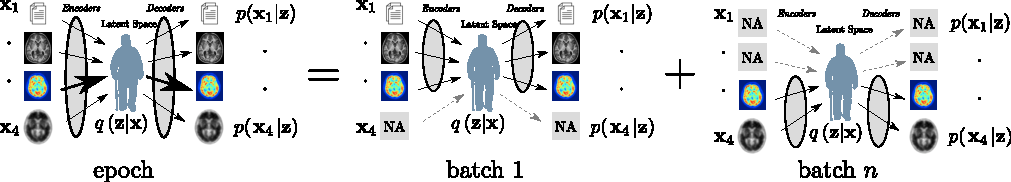
\includegraphics[width=\textwidth]{./tex/fig/model.pdf}
\caption{
Multi-view learning scheme in the presence of missing not available (NA) data.
Arrows represent trainable functions used as network encoders and decoders.
The contribution of datapoints to the model learning is reduced in.
}
\label{fig:model}
\end{figure*}


\subsection{Comparison with VAE and MCVAE}
In \tabref{tab:mcvae} we show how our Multi-Task model extends the capabilities of the Multi-Channel VAE (MCVAE, \cite{Antelmi2019}), which is itself a multi-view extension of the VAE \citep{Kingma2013,Rezende2014}.

In our former work we proposed a multi-view generative model trainable only with observation in the training set have all the available views, limited to model one dataset at a time (in the case of datasets with multiple views), after having discarded incomplete observations in that dataset.
We address this limitation by allowing missing views in the training set for some observations, thanks to the \textit{ad hoc} optimization scheme in \eqnref{eq:argmax}.
\begin{table}[h]
\centering
\caption{
	The Multi-Task Multi-Channel VAE (MT-MCVAE) extends the MCVAE, which is itself an extension of the VAE.
}
\label{tab:mcvae}
\resizebox{\columnwidth}{!}{
	\begin{tabular}{lccc}
	\toprule
		Method                          &  Train with missing data  &  Test with missing data  &  \# views modeled  \\
	\midrule
		VAE       &  no   &  no   &  $1$   \\
		MCVAE     &  no   &  yes  &  $>1$  \\
		MT-MCVAE  &  yes  &  yes  &  $>1$  \\
	\bottomrule
	\end{tabular}
}
\end{table}


As in the MCVAE, at test time, the trained MT-MCVAE model can estimate missing views $\hat\xb_{d,n,v}$ from the available ones through the formula:
\begin{equation}\label{eq:reconstruction}
\begin{aligned}
\hat\xb_{d,n,v} = \frac{1}{V_{d, n}-1} \sum_{w=1, \,w\neq v}^{V_{d, n}} \EE{q_{d,n,w}(\z)}{\p{\xdnv|\z, \thetab_v}},
\end{aligned}
\end{equation}
where the available views $\xdnw$ are encoded into the distributions $q_{d,n,w}$, which are then used to predict the missing view through its decoding distribution $\p{\xdnv|\z, \thetab_v}$.

\subsection{Parameterization}
\label{ssec:parameterization}

With the right choice of the functional form of $\q{\z|\x_{d,n,w}, \phib_w}$, $\pz$, and $\p{\xdnv|\z, \thetab_v}$, the \rhs\ of \eqnref{eq:newLB} becomes amenable to computation and optimization, yielding to the maximization of the \lhs, quantity also known as the model evidence.
Of course, the choice for the likelihood function $\p{\xdnv|\z, \thetab_v}$ depends on the nature of the view $\xdnv$.
For example it can be parametrized as a multivariate Gaussian in the case of continuous data (\ie imaging derived phenotypes), as a Bernoulli likelihood for dichotomic data, and as a Categorical likelihood for categorical data.

In general, the prior distribution $\pz$ is the  multivariate Gaussian distribution $\Gausstd$.
The same family of distributions is also commonly used for the variational and likelihood functions, such that respectively:
\begin{alignat}{4}
\label{eq:encoder}
\q{\z|\xdnw, \phib_w}  &= \mathcal{N} \left( \mub = \mathbf{V}_w^{(\mu)} \xdnw \right. &&{}; &&\left.\Sigmab = \diagp{\mathbf{V}_w^{(\sigma)} \xdnw} \right), \\
\label{eq:decoder}
\p{\xdnv|\z,\thetab_v} &= \mathcal{N} \left( \mub = \mathbf{G}_v^{(\mu)} \zb \right. &&{} ; &&\left.\Sigmab = \diagp{\mathbf{g}_v^{(\sigma)}} \right),
\end{alignat}
where the moments $\mub$ and $\Sigmab$ are obtained from linear transformations of the conditioning variables.
Here, $\thetab_v = \{\mathbf{G}_v^{(\mu)}, \mathbf{g}_v^{(\sigma)}\}$ and $\phib_w=\{\mathbf{V}_w^{(\mu)}, \mathbf{V}_w^{(\sigma)}\}$ are the parameters to be optimized.
A non-linear parameterization can be used as well, for example in the form of deep neural networks.

In \cite{Antelmi2019} we also introduced the following alternative parameterization for the posterior distribution:
\begin{equation}
\label{eq:dropout_posterior}
    q_{d,n,w}(\z) = \Gauss{\mub = \mathbf{V}_w^{(\mu)} \xdnw}{\Sigmab = \diagp{\sqrt{\alphab} \odot \mub^2}},
\end{equation}
which is known as \textit{dropout posterior} \citep{Kingma2015}.
The dropout parameter $\alphab$ has components $\alpha_i = \nicefrac{p_i}{1-p_i}$ linked to the probability $p_i$ of dropping out the $i$-th latent variable component \citep{Wang2013}.
It has been shown that the association of this dropout posterior with a log-uniform prior distribution $\pz$ leads to sparse and interpretable models \citep{Antelmi2019,Molchanov2017}.

